\documentclass[10pt,twocolumn]{article}

\usepackage[latin1]{inputenc}
\usepackage{amsmath}
\usepackage{amsfonts}
\usepackage{amssymb}
\usepackage{graphicx}

\oddsidemargin 0.0in
\topmargin 0.0in
\headheight 0.0in
\headsep 0.0in
\textwidth 6.5in
\textheight 9.0in

\begin{document}

\title{SFFS: Single File File System}
\author{Nitay Joffe\\\texttt{njoffe@ucsd.edu}}
\date{March 15, 2007}
\maketitle

\section{Introduction}
This paper describes the design and implementation of SFFS:
Single File File System. The performance is evaluated in
comparison to two other file systems, one Inode based, and the other FAT.

\section{Design and Implementation}
SFFS got its name from the fact that the entire file system lives in a single
file on the backing disk. The design of the file system is based on FFS, an
Inode based file system.

The development of SFFS was steered by one simple goal: to behave
correctly no matter what events occur. Only the simplest abstractions were 
used, and little optimizations were employed. The file system operates in a 
stateless manner, each operation is unique and independent of any others. This 
means that no caching, hashing of paths, or buffers of data are used anywhere. 
SFFS has the bare necessities required to get the job done, and nothing more.

  \subsection{Disk Layout}
  The disk is organized with the superblock at the very beginning, followed by
  the Inodes, and finally the data blocks.
  
  The number of blocks allocated to the Inodes is decided at format time by
  dividing the number of blocks in the disk by 32. Since each file on the file   
  system has a one-to-one correspondence with an Inode, this is also the 
  maximum number of files supported.
  \begin{figure}[h]
    \begin{center}
      \includegraphics[scale=0.35]{disk_layout.png}
      \label{fig:disk_layout}
      \caption{Disk layout.}
    \end{center}
  \end{figure}

  The block size of SFFS is fixed to 512 bytes. This has been hardcoded to meet
  the constraints of the low level disk reading and writing routines used.

  \subsection{Superblock}
  The superblock contains six items:
  \begin{enumerate}
    \item Size of the disk in blocks.
    \item Inode number of the first free Inode.
    \item Block address of the first free data block.
    \item Inode number of the root Inode.\\
          The root Inode is created during the formatting process and will
          always be placed at the beginning of the Inode section. Therefore,
          strictly speaking, this data is not necessary at all. Having it in
          the superblock though means the root Inode is no different than any
          other Inode since something, somewhere, points to it.
    \item Boolean to tell if the disk was unmounted cleanly.
    \item Magic number used to identify SFFS.
  \end{enumerate}

  \subsection{Inode}
  The Inode is the only place metadata information about the block allocation
  of a given file is stored. Every file, or directory, on the disk has an Inode   
  associated with it.
  \begin{figure}[h]
    \begin{center}
      \includegraphics[scale=0.35]{inode.png}
      \label{fig:inode}
      \caption{Structure of an Inode.}
    \end{center}
  \end{figure}
  
  The direct pointers each point to a block of data. There are 12 of them, so
  this supplies the first 6144 bytes in the file.

  The single indirect pointer points to a block of direct pointers. That block
  contains 128 direct pointers since pointers in SFFS are 4 bytes. This adds
  65536 bytes to the file.

  The double indirect pointer points to a block of single indirect blocks.
  Using similar logic as above, this comes out to an additional 8388608 bytes.

  Finally, the triple pointer points to a block of double pointers. The process
  repeats as before, and this adds a further 1073741824 bytes.

  Adding it all up, the maximum file size supported by an Inode in SFFS is
  1082202112 bytes.

  The space reserved for storing the file size, that is the 31 bits at
  beginning, was decided with this number in mind. It also fits nicely with
  one bit left over to label whether the Inode is associated with a regular 
  file or a directory.

  Inodes take up 64 bytes of disk space, therefore 8 of them fit in a block.
  Inodes are numbered sequentially starting at 0, which is the root directory's 
  Inode.

  \subsection{Directory}
  It is important to note that there is nothing special about a directory 
  block, they store data just like a regular file block. A directory is simply 
  another type of file.

  A directory block consists of 16 entries mapping from a path name to an Inode
  number. The path names are up to 28
  characters (bytes) long, and the Inode number is a 4 byte integer.

  \begin{figure}[h]
    \begin{center}
      \includegraphics[scale=0.35]{directory_entry.png}
      \label{fig:directory_entry}
      \caption{Structure of a directory entry.}
    \end{center}
  \end{figure}

  Directory entries are added in a queue manner, but may get out of order
  because of renaming and deletion operations.

  Searching for an item in a directory is a linear process consisting of
  reading entries sequentially until the item is found or the end of
  the directory is reached. Although the directory entries are adjacent within
  a given block, they do not form a list because there are no pointers. The end
  of
  the directory is detected just like the end of any other file, using
  information in the Inode.

  \subsection{Free Space Management}
  SFFS manages free space using two free lists, one for Inodes and the other
  for data blocks. This free list is implemented as a one-way linked list.
  
  The superblock points to the beginning of the Inode free list and data block
  free list. Those free items contain a pointer (the rest of the block is 
  left unused) to the next free item of that type. A special pointer value of
  0xFFFFFFFF is used to mark the end of the list.

  The Inode free list and the data block free list are the same in all respects
  except for one. Since an Inode takes up 64 bytes, there may be up to 8 free
  Inode slots in a block, whereas a data block is either completely free or
  being used. To circumvent this issue and still be able to use a similar 
  structure for the free lists, the Inode free list pointers are written to 
  point to Inode numbers, not block numbers.

  \begin{figure}[h]
    \begin{center}
      \includegraphics[scale=0.35]{free_list.png}
      \label{fig:directory_entry}
      \caption{Free list example.}
    \end{center}
  \end{figure}

  Deleting a file involves three steps:
  \begin{enumerate}
    \item Find the directory entry containing the file and
          remove that entry from the directory. SFFS does not use a flag to 
          mark the entry invalid. Instead, it copies the last entry in the 
          directory to the location of the entry for the file being removed and 
          then decreases the directory by the size of one entry.
    \item Reclaim the Inode by adding it to the Inode free list.
    \item Add all the blocks owned by the file to the data block free list.
  \end{enumerate}

  Directory deletions are not supported by SFFS.

  When appending items to a free list, SFFS adds to the front instead 
  of the back. This is done by writing the address of the first item to the
  new item and rewriting the superblock to point to the new item.
  
  \subsection{Formatting}
  When a disk is formatted, three things occur:
  \begin{enumerate}
    \item The layout of the disk is computed using Figure 1
%    \item The layout of the disk is computed using Figure
%          \ref{fig:disk_layout}
          and the superblock is written with the calculated information.
    \item The Inode free list and data block free list are written.
    \item The root Inode is created and written.
  \end{enumerate}

  \subsection{Disk Crash Recovery}
  SFFS does not handle any data lost from a disk crash. As long as the crash 
  occurs before or after (not during) a given disk read/write operation, 
  the file system will never become corrupt. This assumption is enforced by
  the low level disk access semantics used, so SFFS doesn't have to worry
  about it. All SFFS has to do is use the low level functions to build
  up complex operations that are still safe.

  Ensuring no failure can occur from a disk crash is done by following a simple
  golden rule: never point to anything that might not exist. For example, when
  deleting a file, first the directory entry in the file's parent directory is
  removed. Next the inode for the file is reclaimed. Finally the data blocks
  are freed.

  Doing operations in this sort of order ensures that if anything breaks
  along the way the worst outcome would be a lost file or some unclaimable
  blocks that are not being used. No corruption will occur.

\section{Evaluation}
The performance measurements were created using a domain specific language
developed in Ruby. The Ruby compiler reads in the DSL file describing the
benchmark and produces a set of incredibly repetitive BASH scripts. Those BASH 
scripts are run in parallel on all of the file systems being benchmarked at 
once. The BASH scripts make calls to other Ruby scripts after their work is 
done to scrape the benchmark output and produce graphs automatically.

\begin{figure}[h]
  \begin{center}
    \begin{verbatim}format_size_in_blocks 100000
arguments 10000, 20000, 30000, 40000
title 'delete a file'
x_label 'file size (bytes)'
run do |argument|
  echo 'a' * argument, '1'
  unmount
  mount
  rm '1'
end\end{verbatim}
    \label{code:delete}
    \caption{DSL file describing the delete benchmark.}
  \end{center}
\end{figure}

  \subsection{Formatting}
  \begin{figure}[h]
    \begin{center}
      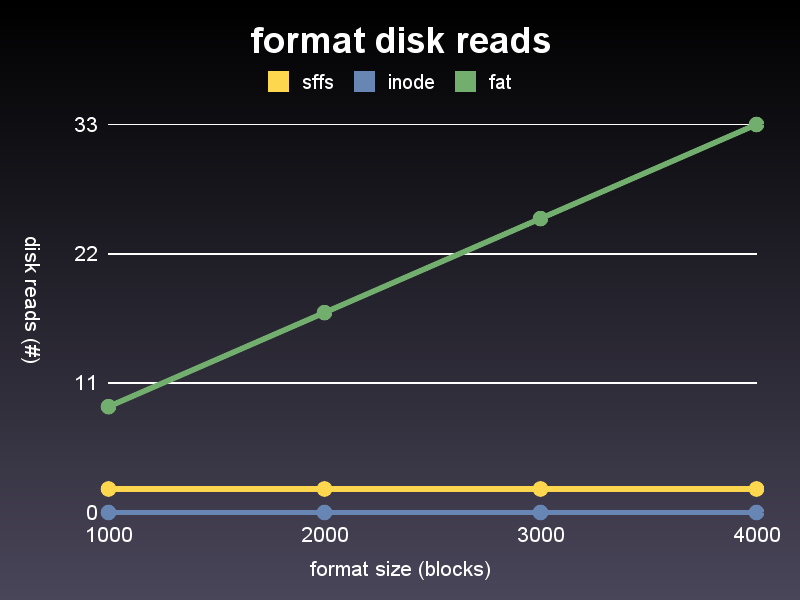
\includegraphics[scale=0.2]{../graphs/format_reads.png}
      \label{fig:delete_seeks}
      \caption{Disk reads for formatting the file system.}
    \end{center}
  \end{figure}

  The interesting point in this graph is that amount of disk reads FAT does 
  increases linearly with the size of the file system being formatted.

  Reading during a formatting operation is completely unnecessary. The user 
  does not have any interaction with disk, so the file system knows about every 
  piece of data that is on the disk. SFFS also does a few unnecessary reads, 
  but the amount remains constant.

  \begin{figure}[h]
    \begin{center}
      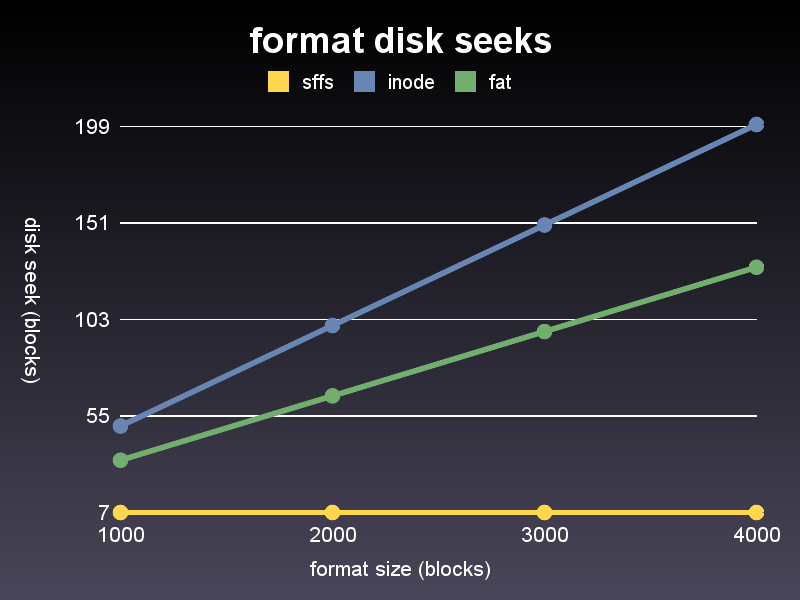
\includegraphics[scale=0.2]{../graphs/format_seeks.png}
      \label{fig:delete_seeks}
      \caption{Disk seeks for formatting the file system.}
    \end{center}
  \end{figure}

  This graph gives insight to the way the formatting is done on the file 
  systems. Both FAT and Inode file systems skip around the disk while doing
  their work. The total movement they make across the disk while formatting is
  linearly dependent on the size of the format.

  SFFS does most of its work in one sweep, which cuts down a lot of disk seek. 
  In particular, when the free lists are written, each block is written to 
  point to the next one in a sequential fashion. Once the write to a block in 
  the free list is finished, the disk head is already in the place of the next 
  one, so no movement needs to happen.

  \subsection{File Read}
  \begin{figure}[h]
    \begin{center}
      \includegraphics[scale=0.2]{../graphs/read_reads.png}
      \label{fig:delete_seeks}
      \caption{Disk reads for reading a file.}
    \end{center}
  \end{figure}

  FAT does a lot of work to read a file, and these results show it. In order to
  read a block of data in a sequential fashion, FAT must first read the table
  entry to find that block. Then it can actually go to that location on disk
  and grab the block. In the process, the location of this block is used to
  find the next block in the file using the table, and the process repeats.
  This process roughly doubles the amount of work required to fetch a block
  from a file.

  Inode based file systems don't need to read in location information for
  every new block they wish to retrieve. The Inode metadata is read in at the
  start, and additional pointer blocks are read in when a boundary between
  pointer types occurs. This process is much more efficient because the
  overhead it adds on stays fairly fixed.

  \begin{figure}[h]
    \begin{center}
      \includegraphics[scale=0.2]{../graphs/read_seeks.png}
      \label{fig:delete_seeks}
      \caption{Disk seeks for reading a file.}
    \end{center}
  \end{figure}

  The benchmark was run from a fresh format, which means the file could be
  written to sequential blocks. This explains the fairly constant seek curves
  for the Inode file systems. FAT still has to go back and forth between the
  actual file blocks and the table as discussed above, so having a localized
  file does not help much with its seek performance.

  SFFS's read curve is steeper than Inode's, which suggests that 
  the Inode file system's internal Inode layout is more efficient.

  \subsection{File Write}
  \begin{figure}[h]
    \begin{center}
      \includegraphics[scale=0.2]{../graphs/write_reads.png}
      \label{fig:delete_seeks}
      \caption{Disk reads for writing a file.}
    \end{center}
  \end{figure}

  The main source of disk reads while writing a file is caused by the search
  for free space. This graph shows that the Inode implementation must be using
  a free list, map, or other sort of data structure that allows an O(1) time
  for finding of a free item. SFFS's free list is O(1) because it just has to
  read the superblock to find the next free item.

  FAT, on the other hand, is doing O(n) searches to find its next free blocks. 
  This suggests that the table is being linearly traversed until a block with a 
  special free marker is found.

  \begin{figure}[h]
    \begin{center}
      \includegraphics[scale=0.2]{../graphs/write_writes.png}
      \label{fig:delete_seeks}
      \caption{Disk writes for writing a file.}
    \end{center}
  \end{figure}

  At first sight this graph should raise a lot of suspicion. As discussed
  previously, FAT operations take about twice as much work to achieve because 
  they have to update the table entry for each block they access. Inodes on the 
  other hand can operate on an entire file and only have to update the 
  associated Inode once. Using this intuition, it is expected that the FAT 
  curve would be roughly twice the slope of Inode/SFFS.

  This expected behavior is not realized because of the internal low level disk
  interface. At the lowest level, disk access can only be done in terms of
  the blocksize, which is 512 bytes. Given this constraint, it is necessary
  to make sure the file system is in a consistent state after every single
  block update.

  SFFS does exactly this by playing it safe and writing an updated inode after 
  every single block write. This adds a lot of overhead, enough to make it 
  behave like a FAT system because it is now writing two blocks for every 
  update. It also means that the amount of data lost during a possible disk
  crash is now reduced to an even finer grain, because each piece of the file
  is protected from the others through this separation.

  As the graph shows, the Inode file system exhibits the exact same behavior.
  It also took the 100\% overhead on each block update which caused it's 
  results to line up so well. This means the Inode file system also plays it
  safe and is consistent during single block updates of a larger write.

  \subsection{File Delete}
  \begin{figure}[h]
    \begin{center}
      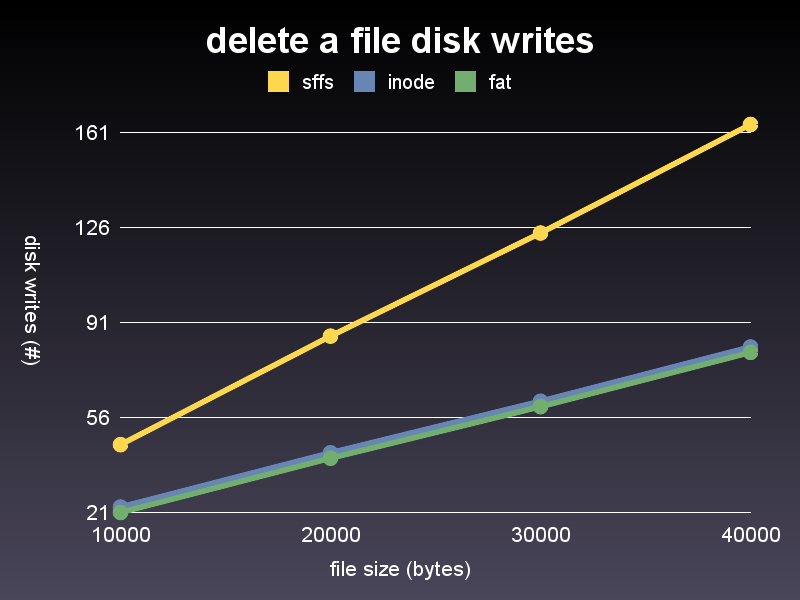
\includegraphics[scale=0.2]{../graphs/delete_writes.png}
      \label{fig:delete_writes}
      \caption{Disk writes for deleting a file.}
    \end{center}
  \end{figure}

  Deletes are substantially more work for SFFS to do than Inode and FAT. This
  is due to the inherently inefficient method of adding free blocks or Inodes
  to the free list.

  As described in the design and implementation section, adding an item to
  a free list comes down to an insert of an item into a linked list. To
  insert that item two updates have to occur, one to make the new item point to
  its successor in the list, and one for the item that is going to point to the 
  newly inserted item. This case is true no matter where in list the new item
  is inserted because even inserting at the end requires writing the end of 
  list marker as the next block pointer.

  \begin{figure}[h]
    \begin{center}
      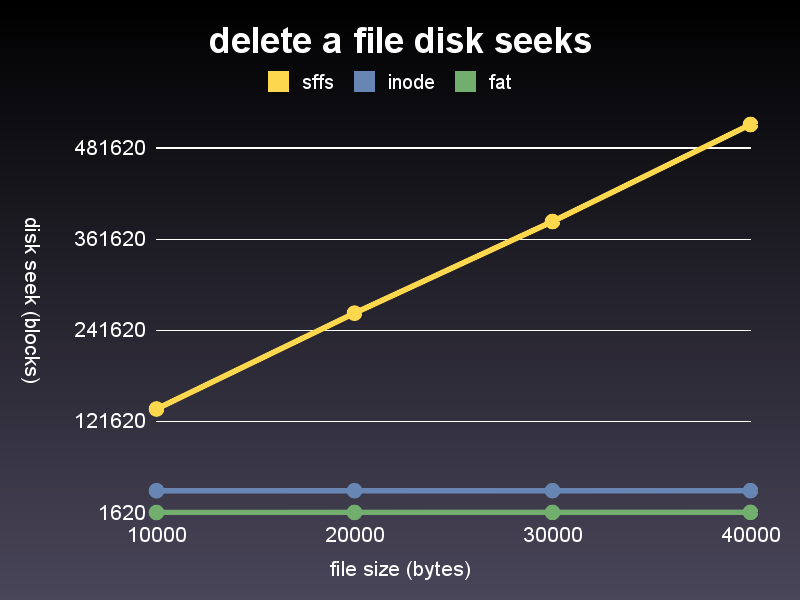
\includegraphics[scale=0.2]{../graphs/delete_seeks.png}
      \label{fig:delete_seeks}
      \caption{Disk seeks for deleting a file.}
    \end{center}
  \end{figure}

  SFFS arbitrarily decided to always insert at the front of the free list. This
  means that every single block or Inode that is freed in the process of a 
  delete requires four steps:
  \begin{enumerate}
    \item Seek to the supernode.
    \item Update the list head to point to the item being freed.
    \item Write a pointer to the item being freed to the supernode.
    \item Seek back to where the work began at.
  \end{enumerate}

  This is a ton of overhead for a block free task to take on, and it adds up
  very quickly when deleting files containing many blocks of data.
   
\subsection{Directory Creation}
  \begin{figure}[h]
    \begin{center}
      \includegraphics[scale=0.2]{../graphs/mkdir_writes.png}
      \label{fig:delete_writes}
      \caption{Disk writes for creating directories.}
    \end{center}
  \end{figure}

  The Inode curve lines up directly with FAT.

  The amount of writing required just to create a directory is the same across 
  all three file systems. They all have to write an entry for the new item in  
  the parent directory and allocate either an Inode or a FAT entry for the new 
  directory.
	
  SFFS incurs a bit more overhead because of its method for allocating blocks
  and Inodes. To allocate an entry, SFFS grabs the head of the free list from
  the superblock. In order to do this, it has to write the pointer contained
  in that entry (the second item in the list) to the superblock. 

  FAT and Inode file systems both use flags to mark free blocks, so overwriting 
  the flag with the data needed also takes care of marking it used.

  \begin{figure}[h]
    \begin{center}
      \includegraphics[scale=0.2]{../graphs/mkdir_seeks.png}
      \label{fig:delete_seeks}
      \caption{Disk seeks for creating directories.}
    \end{center}
  \end{figure}

  SFFS has to seek more than the FAT and Inode file systems because it has to
  update the superblock for each new Inode it allocates. This constant back
  and forth movement to the superblock adds up and creates a lot of disk seek
  overhead.

  This is similar to the seek behavior seen in the file delete benchmark above. 
  The main difference here is that the FAT and Inode file systems' seeks also 
  increase because they have to do more work to find a free block.

\bigskip\bigskip\bigskip
The graphs that are not shown (e.g. disk writes during a file read) were 
omitted because they offered little comparative information. 

Benchmarks for disk crashes were not performed because SFFS does not use any
recovery mechanism.

\section{Conclusion}
The design and implementation of SFFS: Single File File System was presented.
Its performance was discussed using FAT and Inode based file systems for 
comparison.

Using the simplest abstractions and little optimization aided in SFFS's goal of 
correctness no matter what the environment, but it also hindered the 
performance substantially.

Future research and development work to improve the performance of SFFS could
include adding a block level cache, a hash table for quick lookup of Inode
numbers from a path, and a more efficient free space management technique.

The entire free list can be buffered in memory so that batch operations can 
occur. Using this buffer means reallocated items could be inserted in a 
location that is determined to be spatially close to them rather than always 
going to the beginning of the list. Alternative approaches like a free map 
instead of a list can also be helpful.

Lastly, the disk layout can be modified so that Inodes and data blocks are
intermixed. This is similar to the cylinder group idea in FFS and could greatly
reduce the amount of seek overhead as long as file data is placed close to its
corresponding Inode.

\end{document}
